\documentclass[12pt, oneside]{book}
\usepackage{geometry}                		% See geometry.pdf to learn the layout options. There are lots.
\geometry{a4paper}                   		% ... or a4paper or a5paper or ... 
%\geometry{landscape}                		% Activate for rotated page geometry
%\usepackage[parfill]{parskip}    		% Activate to begin paragraphs with an empty line rather than an indent
\usepackage{graphicx}				% Use pdf, png, jpg, or eps§ with pdflatex; use eps in DVI mode
								% TeX will automatically convert eps --> pdf in pdflatex		
\usepackage{amssymb}
\usepackage{fancyhdr}
\usepackage{color}
\usepackage[latin1]{inputenc}
\usepackage{amsmath}
%SetFonts

%SetFonts


\pagestyle{fancy}
\begin{document}
\thispagestyle{empty}
\begin{figure}
\centering%
\includegraphics[scale=0.75]{copertina.jpg}%
\end{figure}
\clearpage
\thispagestyle{empty}
\hspace{10cm}
Release date 26-02-2016
\\
\\
\begin{center}
{\huge Software Engineering 2:}
{\huge MyTaxiService}
\end{center}
\vspace*{\fill}
\begin{center}
\textbf{\huge Requirements Analysis and Specifications Document} 
\\
\large{V2.0}
\end{center}
\vfill % equivalent to \vspace{\fill}
\begin{center}
{\large Dimitar Anastasovski, Marco Colombo}
\end{center}
\clearpage
\pagestyle{plain}
\tableofcontents
\setcounter{page}{1}
\clearpage
\chapter{Introduction}
\section{Purpose}
This document is intended to help understand and communication of the requirements of the system, explaining both the application domain and the system that you want to accomplish. It explains the functional features of the MyTaxiService, along with interface details, design constraints and related considerations such as performance characteristics. It can be considered as a contract between the developer and the customer. 
It is the basis for the planning of the project and to estimate its duration and its cost. It is the base for the activities of testing, verification and validation. The RASD should in fact contain sufficient information to verify if the final system actually satisfies the requirements contained in the document itself. This document follows the IEEE standard for software requirements specification documents. 
\subsection{Intended audience}
This document is intended for all individuals participating in and/or supervising the project:
\begin{itemize}
\item Expected audience of this document is the developers and anyone who intends to develop on this program
\item Developers who can review project's capabilities and more easily understand where their efforts should be targeted to improve or add more features to it (it sets the guidelines for future development). 
\item Project testers can use this document as a base for their testing strategy as some bugs are easier to find using a requirements document. This way testing becomes more methodically organized.
\item End users of this application who wish to read about what this project can do.
\end{itemize}
\section{Scope}
The main accent is to simplify and optimize the access of passengers to the system and to guarantee fair management of taxi queues. We will build flexible and user-friendly web application and a mobile application that will run on Android and IOS mobile phones. This application can be used by anyone who previously will be register on the registration page. After the registration is done the user will have a user name and password that should remember for furthermore usage of the system. The passenger can call a taxi after a successful logging on the application. After that he can call a taxi and he will be informed about the code of the incoming taxi, waiting time. On the other hand taxi drivers will have a mobile application where the major purpose will be to inform the system about their availability, confirmation of a certain call and global map navigation.  City is divided into taxi zones that are uniquely associated with corresponding taxi queues for efficient usage of the system. 
\section{Goals}
We think that the system has to provide this features:
\newline
[G1] Only registered users can use the service - high priority
\newline
[G2] Registered users can use service if and only if they are logged in - high priority 
\newline
[G3] Only eligible users approved by administration can become taxi drivers - high priority 
\newline
[G4] Users can request taxi - high priority 
\newline
[G5] Users can reserve taxi - high priority 
\newline
[G6] Users can cancel a ride - high priority 
\newline
[G7] Checking taxi availability - high priority 
\newline
[G9] Confirming/declining a ride (taxi driver) - high priority 
\newline
[G10] Taxi driver's availability can be changed - high priority 
\section{Abbreviations}
\begin{itemize}
\item ETA: Estimated Time of Arrival, approximated time of arrival of taxi vehicle to destination
\item Reservation: Passenger request for a vehicle at least 2 hours before ride
\item Request: Passenger filled form for immediate ride
\item Reservation Confirmation: Notification sent to the user about the confirmed ride with informations about it
\item Ride Confirmation: Notification sent to the user about the confirmed ride with informations about it
\item User: A person already registered and logged into the application
\item Guest: A person accessing a system that has either never registered or has not logged in yet. Guest has only two available options: log in or register for the first time.
\item Taxi Driver: A person already register and logged into the system as a driver
\item GPS: Global Positioning System
\item API: Application Programming Interface
\end{itemize}
\section{Acronymous}
\begin{itemize}
\item IEEE Standard 830-1998 Recommender Practice for Software Requirements Specifications
\item Specification Document: myTaxiService Project 
\end{itemize}
\section{Document overview}
This document is divided in four parts with clean and non-ambiguity description of the whole system.
\begin{itemize}
\item Chapter 1: General description and basic informartion of the system
\item Chapter 2: Explanation of the main functionalities with constraints, assumptions and hardware dependencies.
\item Chapter 3: Specifications of the system functionalities and non-system functionalities possible scenarios
\item Chapter 4: Use cases and UML models
\item Chapter 5: Alloy modelling and generated world
\end{itemize}
\chapter{Overall description}
\section{Product perspective}
MyTaxiService is a mobile application (Android and iOS) and web application that require users to have access to a web browser on their smartphone or personal computer. The concept is based on the idea of establishing a direct connection between drivers and passengers to offer both sides a modern alternative to conventional booking processes.  After research on the market we will provide unique system for booking a taxi that will benefit customers with cheap fast and satisfying usage of the system.
\section{The world and the machine}
\begin{figure}[h]
\centering
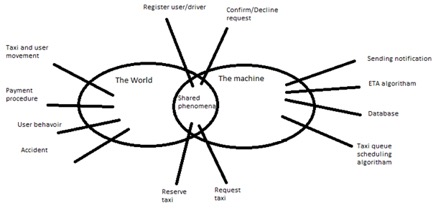
\includegraphics[scale=0.75]{worldmachine.jpg}%
\end{figure}
The world - these activities are initiated by the user or driver or by their environment
\begin{itemize}
\item Taxi movement - happens in user environment
\item Payment - happens between user and driver without accessing the application
\item Accident - can be caused by another vehicles in traffic user environment
\item User behavior - can change the actual state
\end{itemize}
The machine - these activities are used in the system, transparent to users
\begin{itemize}
\item Sending notifications - those actions are initiated by the system, does not include user actions
\item ETA algorithm - is performed by the system
\item Taxi queue and schedule algorithm - is used to efficiently find available taxi vehicle from queue of user's current zone
\item Database - is located in the server side where all datas are stored
\end{itemize}
Shared - these activities require both user and system actions to be completed
\begin{itemize}
\item Request taxi - first, user has to specify origin of the ride and send to system , then system needs to find available taxi driver to complete request
\item Reserve taxi - user has to specify meeting time, origin and destination of the ride, then the system needs to find a taxi vehicle. After that, reservation is completed.
\item Register user/driver - requires user to fill the form that will be sent to the system, which creates user's profile and send back the confirmation message.
\item Confirm decline request - involves user and system. System sends proposal of the ride and then user can choose whether to confirm or decline a ride
\end{itemize}
\section{Product functions}
\begin{itemize}
\item \textbf{Registration: } a guest user can register as passenger:
the user will be able to insert his information such as: first name, last name, e-Mail, phone number, credit card and date of birth.
\\
\item \textbf{Request Taxi: } after the request, the system will report the amount of the trip to the passenger and he can proceed with the payment. After that according to the informations provided by the passenger, the system will have to alert the closest driver in the queue of the desired zone.
\\
\item \textbf{Reserve taxi: }passengers can reserve a taxi at least 2 hours before the desired time. After the reservation, a taxi will be allocates to the request 10 minutes before the meeting time. 
\end{itemize}
\section{User characteristic}
We expect massive usage from people who use public transport on a daily basis regardless age, gender and nationality. Expected users must have basic knowledge of using web browser and have access to internet.
\begin{itemize}
\item \textbf{Guest: }a person that has not registered and can only exploit basic functionalities such as looking for help. 
\item \textbf{User: }a person that has registered and has provided his personal information and a set of abilities. 
\begin{enumerate}
\item Passenger
\item Taxi driver
\end{enumerate}
\item \textbf{Administrator: }the responsible for the web application. The only one that can accept new abilities from users. 
\end{itemize}
\section{Constraints}
Mayor constrains are related to security and reliability of the system and customers. The Service may admit you to link to other websites, services or resources on the Internet, and other websites, services or resources may contain links to the Site. When you access third party websites, you do so at your own risk. These other websites are not under our control. 
\begin{itemize}
\item Regulatory polices harmonized with Italian regulatory agency.
\item Hardware and software limitations 
\end{itemize}
\begin{tabular}{|c|c|}
\hline
  & {Requirements} \\
\hline
\makebox[5cm][c]{Operating system} &\makebox[10cm][c]{Windows(XP or higher), }\\
& Linux(Edubuntu,Ubuntu or higher),\\
& Mac OS (X 10.6 or higher), \\
& Android(Froyo or higher), iOS( 7.0 or higher) \\
\hline 
CPU & 1.5Ghz or higher\\
\hline
Memory & 512 MB�RAM(for PC)\\
& 32 MB RAM (for Android and iOS)\\
\hline
Hard drive & 2.2 GB free�hard disk�space\\
\hline
Browser requirements & \makebox[9cm][c]{Internet explorer 6 or higher, Google Chrome,} \\
& Mozila Firefox, Apple Safari 5+ \\
\hline
GPS & YES \\
\hline
Internet Connection & YES \\
\hline
\end{tabular}
\begin{itemize}
\item Interfaces to other applications:
\\
MyTaxiService doesn't meet with other application 
\item Parallel operation: 
\\
MyTaxiService must support parallel operations
\item For testing purposes you will need a simulating tool. 
\end{itemize}
\section{Assumptions and dependencies}
\begin{itemize}
\item If you close the application the reservation of the taxi continues, push notification will be send before the taxi arrives.
\item Administrator (or the system) has authority to delete account
\item Customer can only reserve taxi at least two hours before the ride
\item Taxi driver can receive ride request while he is unavailable
\item Taxi driver that is currently on ride can't receive requests
\item Only available taxi drivers can receive ride requests
\item Taxi driver can cancel the reservation
\item User can only have one account
\item If customer had more than three cancellation, administrator (or the system) can block his account
\item Customer can reserves maximum three taxis
\item Customers can cancel reservation, but the system must inform the taxi driver
\item Special code must send with the reservation for easily recognition by the customers
\item MyTaxiService can be only use in Milan (including Malpensa and Linate airports)
\item If in the concrete zone there are no available taxis in the queue, the system can ask the customer if he wants to automatically give the reservation to the closest zone with approximate waiting time and additional cost
\item If there is no available taxi in the zone, customer can see queue of reservation taxis near the customer with approximate waiting time
\item There is a Terms \& Conditions section to indicate clearly the usage of the application, which if not followed will result in account deactivation
\end{itemize}
\clearpage
\chapter{Requirements}
Starting from the goals we explain the following requirements:
\begin{enumerate}
\item \textbf{Allow the registration in the application to taxi drivers and passengers:}
\begin{itemize}
\item The system should be able to provide a sign up functionality in order to create a new taxi driver or passenger profiles.
\end{itemize}
\item \textbf{Simplify the access of passengers to the taxy service:}
\begin{itemize}
\item The system has to provide the possibility to the passenger to reserve a taxi
\item The system has to provide both a web application and mobile application in order to allow the passenger to save his time.
\end{itemize}
\item \textbf{Allow passenger to view if there is any taxi driver free:}
\begin{itemize}
\item The system has to provide a functionality that allow a passenger to view if there is any free taxi driver for the desired route.
\end{itemize}
\item \textbf{Divide the city into different areas covered by some taxi drivers, organized in queues:}
\begin{itemize}
\item The system has to provide a functionality to divide the city in some areas
\item The system has to organize the taxi of these areas into queues
\end{itemize}
\item \textbf{Guarantee a fair management of taxi queues:}
\begin{itemize}
\item The system has to provide a functionality in order to manage the taxi queues in the best way possible.
\end{itemize}
\item \textbf{Allow the client to reserve taxi for an exact time:}
\begin{itemize}
\item The system has to provide a functionality that allow the passenger to reserve a taxi for a desired time.
\end{itemize}
\end{enumerate}
\section{Functional requirements}
We specify here functional requirements for each actor:
\begin{enumerate}
\item \textbf{Guest:}
\begin{itemize}
\item Sign up
\end{itemize}
\item \textbf{Passenger:}
\begin{itemize}
\item Log in
\item Manage personal informations
\item Request a taxi
\item Reserve a taxi
\end{itemize}
\item \textbf{Taxi driver:}
\begin{itemize}
\item Log in
\item Manage his personal informations
\item Share his position on the map
\item Change his status (free or busy for a ride)
\end{itemize}
\end{enumerate}
\clearpage
\section{External interface requirements}
\subsection{User interface}
\vspace{2cm}
\hspace*{\fill}
\textbf{\large Homepage \& registration page}
\hspace*{\fill}
\begin{figure}[h]
\includegraphics[scale=0.7]{Homepage.png}
\end{figure}
\\
The passenger can access to the registration page and register himself to the application.
\clearpage
\hspace*{\fill}
\textbf{\large Login}
\hspace*{\fill}
\begin{figure}[h]
\centering
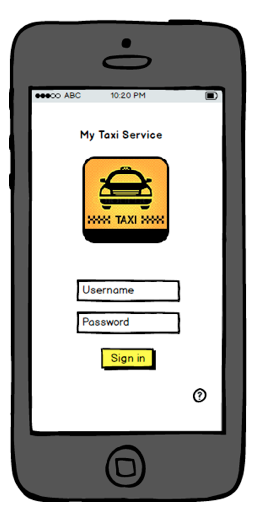
\includegraphics[scale=0.7]{login.png}
\end{figure}
\\
This is the login page. Here the user after entered his data can sign in the application.
\vspace{1cm}
\clearpage
\hspace*{\fill}
\textbf{\large Menu}
\hspace*{\fill}
\\
\begin{figure}[h]
\centering 
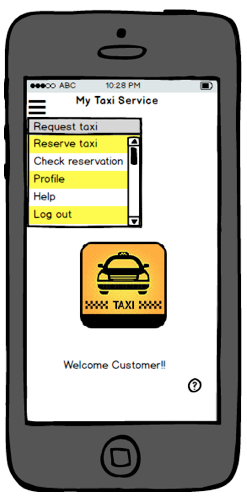
\includegraphics[scale=0.7]{menu.png}
\end{figure}
\\
This is the menu page, here the user can navigate and choose what to do. There are several options like: reserve taxi, check reservation, profile, help or log out.
\clearpage
\hspace*{\fill}
\textbf{\large Reservation}
\hspace*{\fill}
\\
\begin{figure}[h]
\center 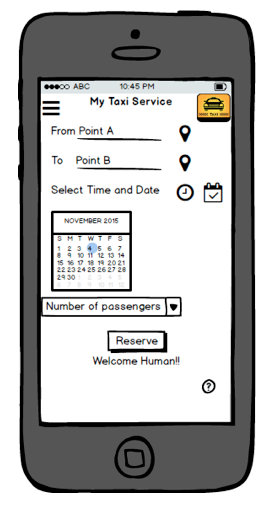
\includegraphics[scale=0.7]{reservation.png}
\end{figure}
\\
Here the passenger can reserve a taxi. He needs to insert the starting and destination point, the date and the number of passenger.
\clearpage
\hspace*{\fill}
\textbf{\large Confirm reservation}
\hspace*{\fill}
\\
\begin{figure}[h]
\center 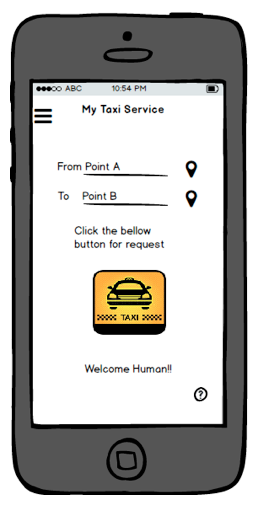
\includegraphics[scale=0.7]{confirmreservation.png}
\end{figure}
\\
In this page the passenger can show a recap of his trip and confirm the reservation by clicking on the button
\clearpage
\hspace*{\fill}
\textbf{\large Recap reservation}
\hspace*{\fill}
\begin{figure}[h]
\center 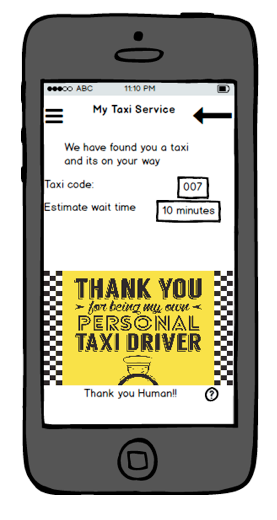
\includegraphics[scale=0.7]{recapreservation.png}
\end{figure}
\\
Here the passenger can see the estimate waiting time and the code of the taxi that will pick him up.
\clearpage
\hspace*{\fill}
\textbf{\large Taxi driver homepage}
\hspace*{\fill}
\\
\begin{figure}[h]
\center 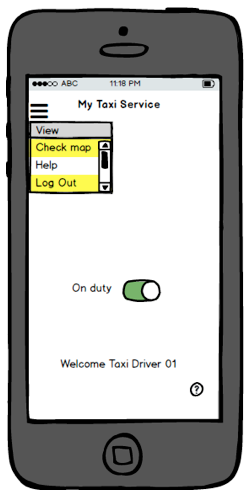
\includegraphics[scale=0.7]{taxidriverhome}
\end{figure}
\\
This is the home page for the taxi driver. He can choose from different option such as: Check map, Help or Log out. Also he can change his status in busy or free.
\clearpage
\hspace*{\fill}
\textbf{\large Taxi driver request}
\hspace*{\fill}
\\
\begin{figure}[h]
\center 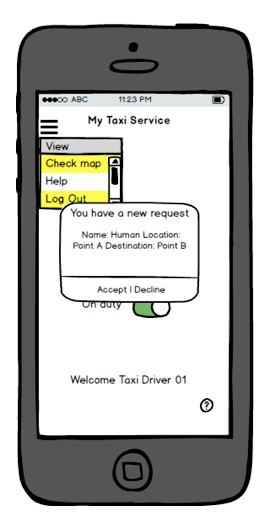
\includegraphics[scale=0.7]{taxirequest}
\end{figure}
\\
This is the notification that the taxi driver will receive when there is a request of a taxi. He can choose if accept or decline this request.
\clearpage
\hspace*{\fill}
\textbf{\large Reservation list for taxi driver}
\hspace*{\fill}
\\
\begin{figure}[h]
\center 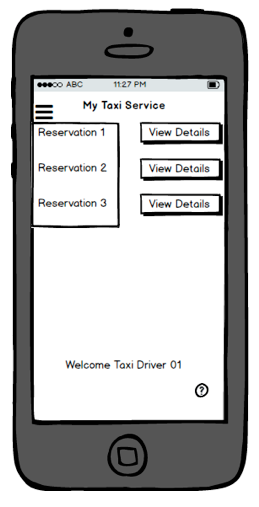
\includegraphics[scale=0.7]{reservationlist}
\end{figure}
\\
Here the taxi driver can give a look at the reservation he has in list and its details.
\clearpage
\hspace*{\fill}
\textbf{\large Taxi driver map}
\hspace*{\fill}
\\
\\
\begin{figure}[h]
\center 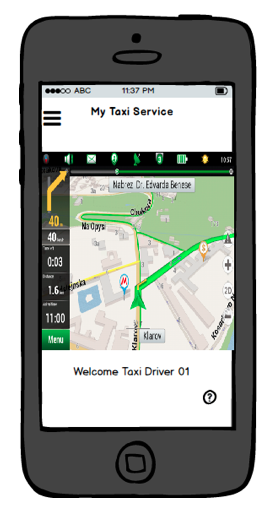
\includegraphics[scale=0.7]{taxidrivermap}
\end{figure}
\\
In this page the taxi driver can see the map of the itinerary for the reservation he chooses.
\clearpage
\subsection{Software interface}
Our software will have a database which saves members then serve a data management. In order to verify the data for the taxi drivers, the system must have access to the police database through and verify data on driving license and car. Enabling you to record your credit card the system will use bank pass that allows you to check the validity of information, the software have to use the maps google.
\section{Scenarios}
\begin{itemize}
\item \textbf{\large Scenario 1}
\\
Alan has to leave for a trip in Milan and there is no one on arrival who can get him. Helping with his smartphone, he connects to myTaxiService app and does the log in using his data created in the registration phase. He requests a taxi in that area. In few minutes Alan is in the taxi and can get where he wants to lead.
\item \textbf{\large Scenario 2}
\\
Alan has to leave for a business trip in Milan and on arrival he must be at an appointment in less that an hour. Alan makes the access to the myTaxiService application, does the log in with his datas and makes a reservation for a taxi at the arrival time in Duomo. Now Alan can make the trip with tranquility and will not miss his appointment.
\item \textbf{\large Scenario 3}
\\
Mario is a taxi driver and he received a request for a ride, he accessed the app and change his status from free into busy. When he will finish the ride, he will change the status into free and waits for the next call.
\item \textbf{\large Scenario 4}
\\
Mario is a taxi driver and he must be at the Linate airport to pick up Alan at the arrival. During the travel the car has a problem and stops to work. Mario immediatly try to repair the car but there isn't anything to do. He sends a notification to Alan and cancel the reservation. Alan will be refunded on his credit card.
\item \textbf{\large Scenario 5}
\\
Luca heards a friend talking about MyTaxiDriver App so he decided to download it and use it because he need to make a reservation for the next day. After the download he registers himself into the application and in few minutes he is ready to go. He logs in and make the reservation. The next day he will find the taxi cab at the desired point.
\end{itemize}
\section{Nonfunctional requirements}
\subsection{Reliability}
\begin{itemize}
\item Application must provide real time driver availability information.
\item Application must provide accurate estimate time arrival of the driver.
\item Application must provide accurate estimate fare.
\item Application must send the booking request to the licensed taxi drivers.
\end{itemize}
\subsection{Availability}
\begin{itemize}
\item Application must serve the customers 24 hours, 7 days in a week.
\end{itemize}
\subsection{Security}
\begin{itemize}
\item The system must use encryption to protect the customers and the drivers. 
\end{itemize}
\subsection{Usability}
\begin{itemize}
\item User friendly interfaces (intuitive and easy to use)
\item Fast access to content, information (in case of numbers request to the server)
\item Presenting data and information?s  in clear, logical and readable way.
\end{itemize}
\subsection{Maintainability}
\begin{itemize}
\item The program must be designed in a way that new addition can be done without changing
the already developed structure.
\end{itemize}
\subsection{Portability}
\begin{itemize}
\item MyTaxiService is completely portable. 
\end{itemize}
\subsection{Future implementation}
\begin{itemize}
\item Customers can use the option taxi sharing
\item More available operating zones for the taxis
\item You can add favorite drivers
\end{itemize}
\chapter{UML Models}
\section{Use Case Models}
\vspace{2cm}
\begin{figure}[h]
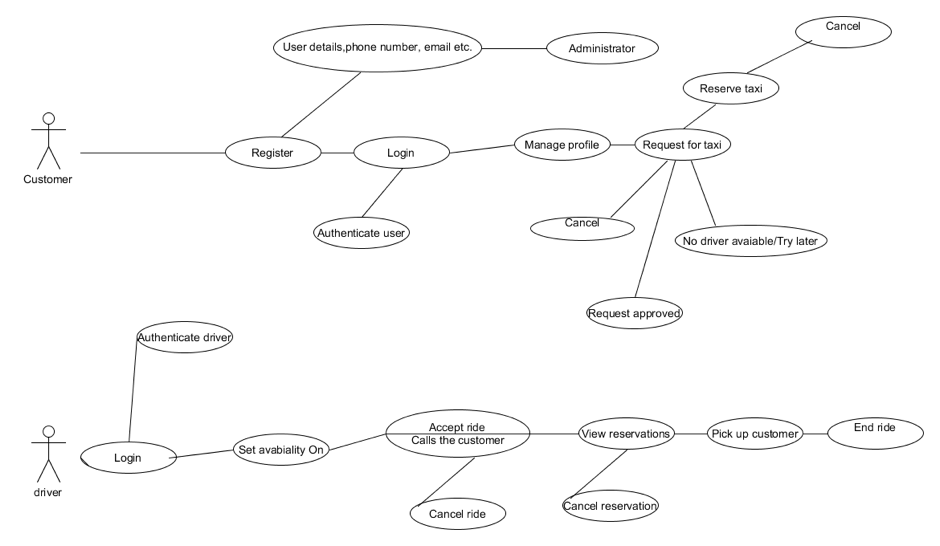
\includegraphics[scale=1]{general.png}
\end{figure}
\clearpage
\begin{figure}[h]
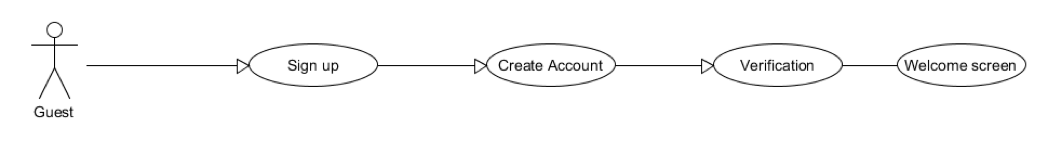
\includegraphics[scale=0.8]{signup.png}
\end{figure}
\vspace{3cm}
\begin{tabular}{|l|l|}
\hline
Name & \textbf{Sign up} \\
\hline
Actors & Guest \\
\hline
Entry conditions & Guest never made profile to our system \\
\hline
& Guest is clicking on the registration form. \\
&The system shows to the guest the registration form \\
Events flow&where he needs to enter basic require informations \\
& and in the end he clicks sign in. \\
&The system checks if the informations are valid, \\
&confirms and redirects the guests to the homepage. \\
\hline 
& The informations are stored in the database, \\
Exit conditions &confirmation mail is send \\
&to the guest and the user is redirected to the homepage\\
\hline
Exceptions & If the guest inserts non valid informations \\
&the system shows an error message \\
\hline
\end{tabular}
\clearpage
\begin{figure}[h]
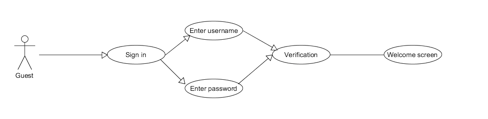
\includegraphics[scale=0.9]{loginusecase.png}
\end{figure}
\vspace{3cm}
\begin{tabular}{|l|l|}
\hline
Name & \textbf{User log in} \\
\hline
Actors & User \\
\hline
Entry conditions & The user wants to log in into the system \\
\hline
& The user navigates to the home screen of the\\
&MyTaxiService.\\
&The system shows login page and the user inserts\\
Events flow&username and password and clicks on\\ 
&the sign in button\\
&The system validate the correctness of the\\ 
&inserted information, confirms and redirects\\ 
&to his personal page\\
\hline 
Exit conditions & The user has access to MyTaxiService functionality \\
\hline
Exceptions & If guest inserts non valid informations the system shows \\
&an error message \\
\hline
\end{tabular}
\clearpage
\begin{figure}[h]
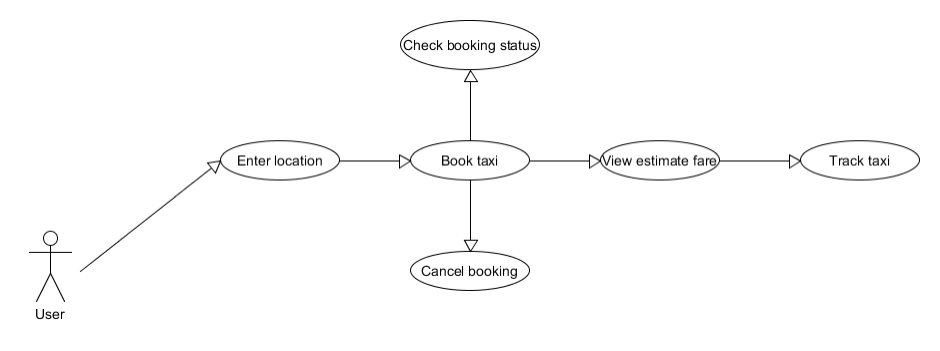
\includegraphics[scale=0.9]{enterlocation.png}
\end{figure}
\vspace{3cm}
\begin{tabular}{|l|l|}
\hline
Name & \textbf{Request for a taxi} \\
\hline
Actors & User \\
\hline
Entry conditions & The user is logged in \\
\hline
& The user choose "Request a taxi" in the homepage \\
&The user is redirected to the page where he enters\\ 
&his location and final destination. And he clicks request.\\
Events flow &After that the GPS is correctly acquired, the user\\ 
&can sent the request tapping the relative button. \\
&A confirmation page appears with the code of the \\
&incoming taxi and the waiting time\\
\hline 
Exit conditions & Code is send to the user and estimate waiting time \\
\hline
& If the users didn't enter his location the system shows \\
Exceptions &an error message and if there is no available taxi the\\
&system shows an error message\\
\hline
\end{tabular}
\clearpage
\begin{figure}[h]
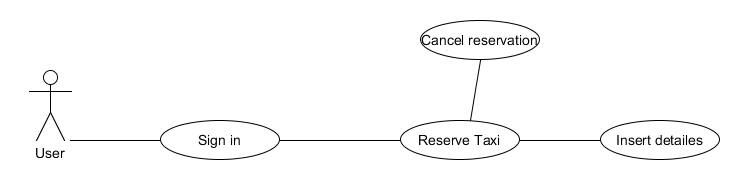
\includegraphics[scale=0.6]{taxireserv.jpg}
\end{figure}
\vspace{3cm}
\begin{tabular}{|l|l|}
\hline
Name & \textbf{Taxi reservation} \\
\hline
Actors & User \\
\hline
Entry conditions & The user is logged in \\
\hline
& The user choose "Reserve Taxi" in the home page\\
&User is redirected to "Reserve Taxi" section where he\\ 
&needs to enter the details for reserving taxi: \\
&\hspace{1cm}\textbf- Meeting location\\
Events flow &\hspace{1cm}\textbf- Favorite destination\\
&\hspace{1cm}\textbf- Date and time for pick up\\
&\hspace{1cm}\textbf- Number of passengers\\
&After entered required fields the user confirms by\\
&clicking the button "Reserve"\\
\hline 
&The user receives confirmation from the system and\\
Exit conditions &a push notification 10 minutes before the meeting time\\
&with the code of the incoming taxi\\
\hline
Exceptions & The user can't reserve taxi at least two hours\\
& before the ride\\
\hline
\end{tabular}
\clearpage
\begin{figure}[h]
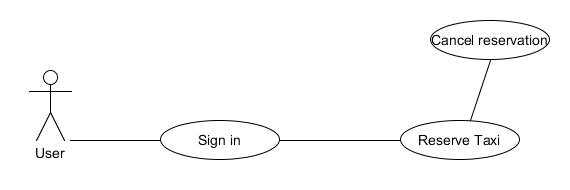
\includegraphics[scale=0.7]{cancelreserv.jpg}
\end{figure}
\vspace{3cm}
\begin{tabular}{|l|l|}
\hline
Name & \textbf{Cancel ride} \\
\hline
Actors & User \\
\hline
Entry conditions & The user is logged in \\
\hline
Events flow & The user goes to "Reserve taxi" option and clicks on\\
&"Cancel reservation"\\
\hline 
Exit conditions & The reservation is properly deleted\\
\hline
Exceptions & The user can't cancel reservation less than 10 minutes\\
&before the taxi arrives\\
\hline
\end{tabular}
\clearpage
\begin{figure}[h]
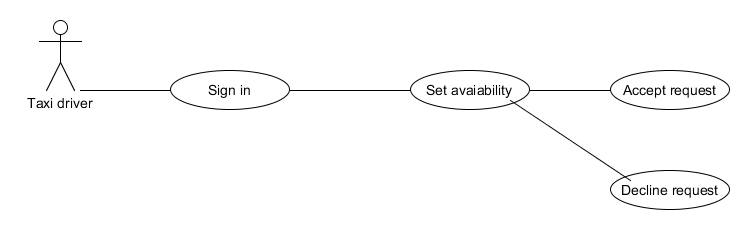
\includegraphics[scale=0.6]{confirmdeclinereuest.jpg}
\end{figure}
\vspace{3cm}
\begin{tabular}{|l|l|}
\hline
Name & \textbf{Confirmation or declined request} \\
\hline
Actors & Taxi driver\\
\hline
& The taxi driver is available, the taxi is the first in\\
Entry conditions&availability queue of its zone, so an available\\
&ride is coming soon\\
\hline
Events flow & The taxi driver is notified for a request and we can\\ 
&accept or declined the request\\
\hline 
& The taxi driver accepts the ride\\
Exit conditions &The taxi driver rejects, the system will move the taxi\\ 
&in the last position of the relative available queue\\
\hline
Exceptions & If the taxi driver has some issues, he need to inform\\
&the administrator.\\
\hline
\end{tabular}
\clearpage
\section{Class Diagram}
Here we represent the class diagram of the entire system
\vspace{4cm}
\begin{figure}[h]
\centering
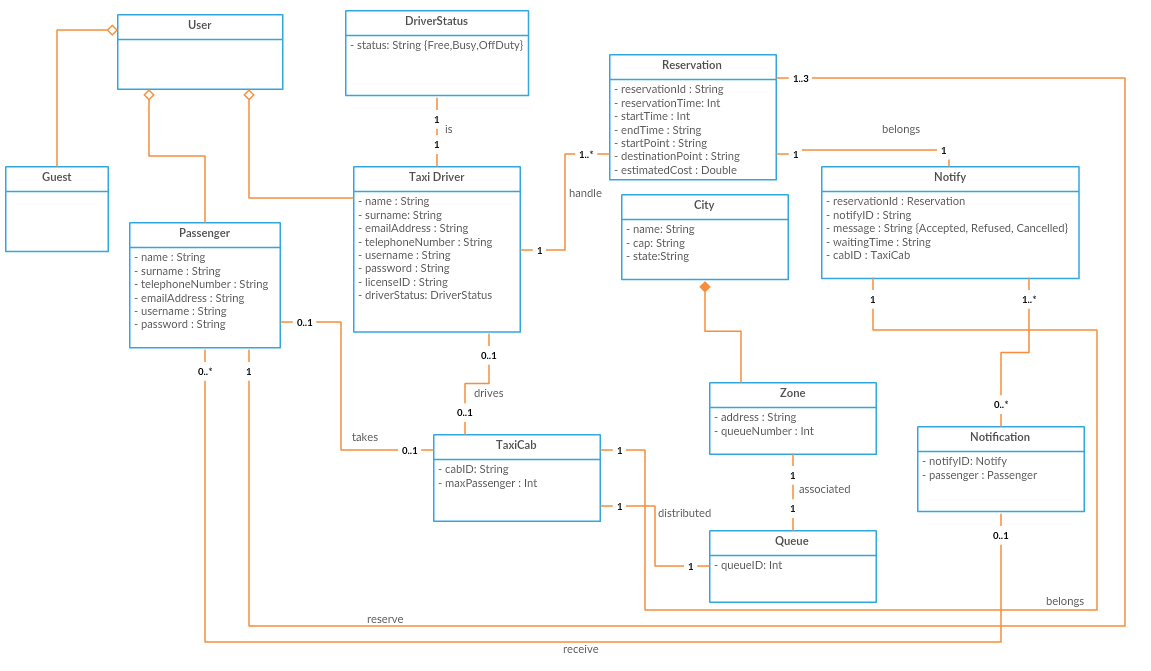
\includegraphics[scale=0.4]{classdiagram2.png}
\end{figure}
\clearpage
\section{Sequence Diagrams}
This is the sequence diagram for the login procedure
\vspace{3cm}
\begin{figure}[h]
\centering
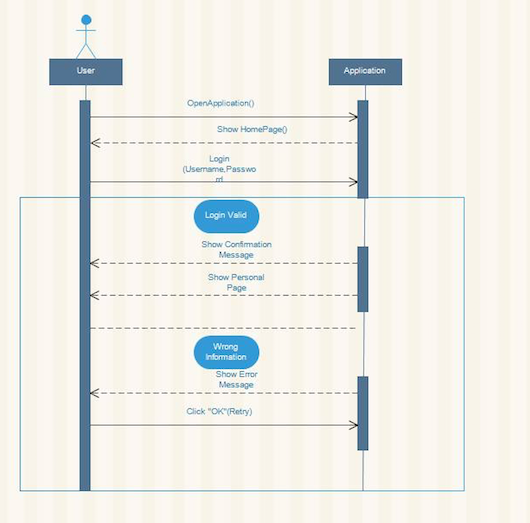
\includegraphics[scale=0.7]{loginsequence.png}
\end{figure}
\clearpage
Here we represent the sequence diagram for the reservation of a taxi
\vspace{3cm}
\begin{figure}[h]
\centering
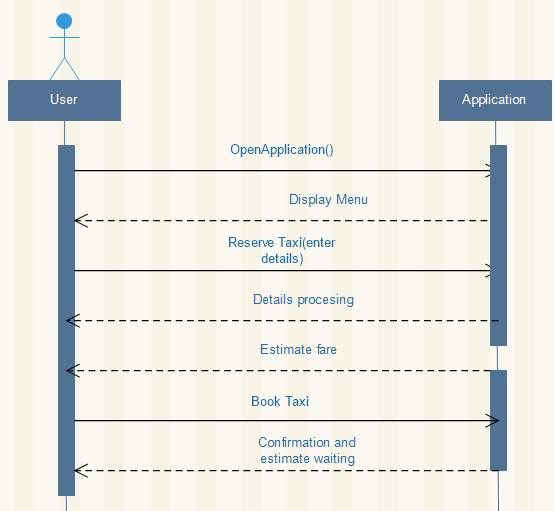
\includegraphics[scale=0.6]{reservetaxi.jpg}
\end{figure}
\clearpage
Here its described the sequence diagram for cancel a reservation
\vspace{3cm}
\begin{figure}[h]
\centering
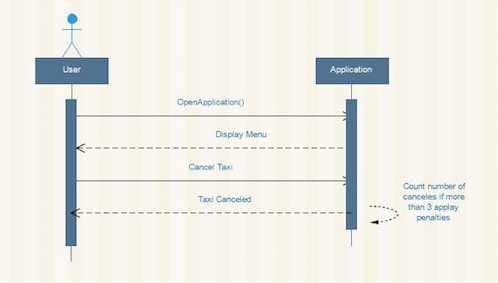
\includegraphics[scale=0.7]{cancelreservation.png}
\end{figure}
\clearpage
\section{Activity diagrams}
\vspace{2cm}
\hspace*{\fill}
\textbf{\large Login}
\hspace*{\fill}
\begin{figure}[h]
\centering
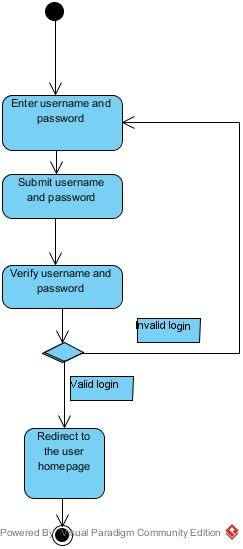
\includegraphics[scale=0.7]{loginactivity.jpg}
\end{figure}
\clearpage
\hspace*{\fill}
\textbf{\large Request}
\hspace*{\fill}
\begin{figure}[h]
\centering
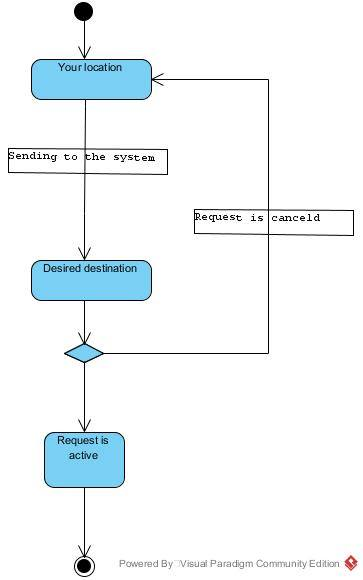
\includegraphics[scale=0.7]{requestactivity.jpg}
\end{figure}
\chapter{Alloy}
\section{Signatures}
\begin{figure}[h]
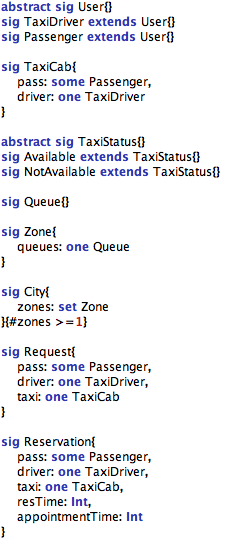
\includegraphics[scale=0.63]{sig.png}
\end{figure}
\clearpage
\section{Facts}
\begin{figure}[h]
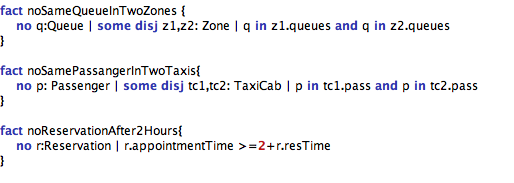
\includegraphics[scale=0.7]{fact.png}
\end{figure}
\section{Predicates}
\begin{figure}[h]
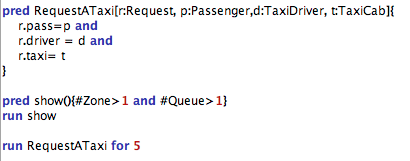
\includegraphics[scale=0.65]{pred.png}
\end{figure}
\section{Results}
\begin{figure}[h]
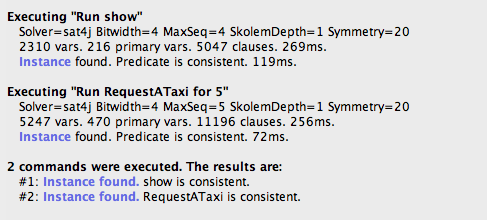
\includegraphics[scale=0.7]{result.png}
\end{figure}
\section{Generated world}
\vspace{1cm}
\begin{figure}[h]
\centering
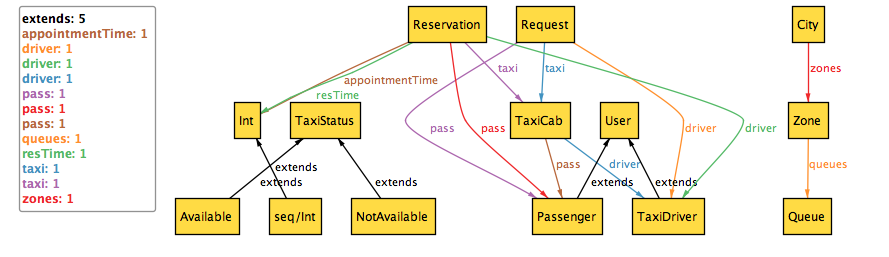
\includegraphics[scale=0.52]{world.png}
\end{figure}
\clearpage
\chapter{Appendix}
\section{Software and used Tools}
\begin{itemize}
\item TexShop (http://pages.uoregon.edu/koch/texshop/): to redact this document
\item Alloy analyzer 4.2 (http://alloy.mit.edu/alloy/): to prove the consistency of the model
\item CreatelyApp (https://creately.com/app/): to create Class diagram
\item Balsamiq Mockups (https://balsamiq.com/products/mockups/): to create the user interface mockup
\item Visual paradigm (http://www.visual-paradigm.com): to create the activity diagrams
\item UMLet (http://www.umlet.com): to create sequence and use case diagrams
\end{itemize}
\section{Working hours}
\textbf{Dimitar Anastasovski:} $\thicksim$35 hours
\\
\\
\textbf{Marco Colombo:} $\thicksim$35 hours
\section{Changelog}
We had changed the alloy parts, the goals and some minor things from the first RAS document.
\end{document}  